% Chapter 4

\chapter{Parallel Predictive Entropy Search For Multi-Objective Bayesian Optimization With Constraints} % Write in your own chapter title
\label{Chapter5}
\lhead{Chapter \ref{Chapter5}. \emph{Parallel Predictive Entropy Search For Multi-Objective Bayesian Optimization With Constraints}} 

{\bf \small{
As we have seen in the previous chapter, real-world problems often involve the optimization of several 
objectives under multiple black-boxes. We have also described how BO can recommend a valid Pareto set
at the end of its execution. A limitation of the described methodology, however, 
is that current BO methods, as PESMOC, for these problems, choose a point at a time 
at which to evaluate the black-boxes. If the expensive evaluations can 
be carried out in parallel (as when a cluster of computers is available), this 
results in a waste of resources. In this chapter, we introduce PPESMOC, 
Parallel Predictive Entropy Search for Multi-objective Optimization 
with Constraints, an extension of PESMOC for solving the problems 
described. PPESMOC selects, at each iteration, a batch of input locations at 
which to evaluate the black-boxes, in parallel, to maximally 
reduce the entropy of the problem's solution. To our knowledge, this is 
the first batch method for constrained multi-objective BO. In this chapter we present 
empirical evidence in the form of synthetic, benchmark and real-world experiments 
that illustrate the effectiveness of PPESMOC.  }}

\section{Introduction}
A limitation of BO methods for constrained multi-objective optimization 
like PESMOC, which was described in the previous chapter, is that they choose a point at a time at which to evaluate the black-boxes. 
Assume that a cluster of computers or some other resource is available to perform the evaluation of the black-boxes at
several points in parallel. If only a single point is evaluated each time, this results in a
a waste of resources and leads to sub-optimal optimization results. The problem described can be
solved by using BO methods that suggest not only a single point at which to evaluate the 
black-boxes, but a batch or collection of points of adjustable size 
\citep{azimi2012hybrid,bergstra2011algorithms,gonzalez2016batch,shah2015parallel}.

To the best of our knowledge, no parallel BO method has been proposed to deal with the optimization of 
multiple objectives under several constraints. Only sequential methods exist. Therefore, the 
literature about BO is missing important methods to address BO problems with the characteristics described. 
In this chapter, we propose a BO method that can precisely address the problems described 
and can suggest, at each iteration, a batch of points at which to evaluate all the 
black-boxes in parallel. The method proposed is based on an extension of the PESMOC method
described in the previous chapter and an extension of sequential constrained 
multi-objective BO \citep{shah2015parallel}. More precisely, the acquisition function that we 
consider receives as an input a batch of candidate input locations at which to perform the evaluation
of the black-boxes in parallel and estimates the expected reduction in the entropy of the solution of 
the optimization problem. The difference with PESMOC is that here, the acquisition function evaluates
a batch of points instead of a single one. 

We have carried out extensive experiments to evaluate the performance of PPESMOC 
in synthetic, benchmark and real-world optimization problems. Furthermore, we have 
compared results with a base-line which chooses the points to evaluate at random 
and with a simple method that applies iteratively  a sequential BO method
for constrained multi-objective BO (as many times as the batch size). 
This last method introduces virtual observations (fantasies) to avoid choosing many times the same point.  
The results show that PPESMOC performs better than a random search strategy and 
similarly or better than sequential base-lines. The advantage of the proposed approach is, 
however, that its cost scales much better with respect to the batch size than the sequential base-lines.

\section{Parallel Bayesian Optimization}

Any sequential BO strategy can be transformed into a batch one by
iteratively applying the sequential strategy $B$ times.  
To avoid choosing similar points each time, one can simply 
hallucinate the results of the already chosen pending evaluations \citep{snoek2012practical}. 
For this, the acquisition function is simply 
updated from $\alpha(\mathbf{x}|\mathcal{D})$ to $\alpha(\mathbf{x}|\mathcal{D} 
\bigcup {(\mathbf{x}_i , \mathbf{h}_i)\,, \forall \mathbf{x}_i \in \mathcal{P}})$, 
where $\mathcal{D}$ are the data collected so far, $\mathcal{P}$ is the set of pending 
evaluations, and $\mathbf{h}_i$ denotes the hallucinated evaluation result for the 
pending evaluation $\mathbf{x}_i$. A simple approach is to update the surrogate model after choosing each 
batch point by setting $\mathbf{h}_i$ equal to the mean of the predictive distribution 
given by the GPs \citep{desautels2014parallelizing}. Of course, this strategy, to which we
refer to as parallel sequential, has the disadvantage of requiring the optimization of the
acquisition $B$ times, and also updating the GPs using hallucinated 
observations. This is expected to lead to extra computational cost than in PPESMOC.

PPESMOC is a generalization of PESMOC, which was described in the previous chapter. PESMOC is 
the current state-of-the-art for solving constrained multi-objective BO problems. 
Nevertheless, PESMOC is a sequential BO method that can only suggest one point at a time to 
be evaluated. It cannot suggest a batch of points as PPESMOC. PESMOC also works by choosing the 
next candidate point as the one that is expected to reduce the most the entropy of the Pareto set in the feasible 
space. The required computations are also approximated using the expectation propagation algorithm \citep{minka2001expectation}. 
Notwithstanding, the extension of PPESMOC over PESMOC is not trivial. In particular, in PPESMOC the 
acquisition function involves additional non-Gaussian factors (one per each point in the batch) and 
requires the computation of its gradients. These are not needed in PESMOC 
as the input dimensionality in that method is smaller, \emph{i.e.}, $D$ vs. $B \times D$.

\section{Parallel Predictive Entropy Search for Multi-Objective Bayesian Optimization with Constraints}

Consider $N$ observations $\mathcal{D}=\{ (\mathbf{x}_i,\mathbf{y}_i)\}_{i=1}^N$
of the black-boxes obtained so far. We define $\mathbf{X}_{N+1}=\{\mathbf{x}_1,\ldots,\mathbf{x}_B\}$ as the 
batch of $B$ points where the black-boxes should be evaluated at the next iteration. In this chapter, we describe
how PPESMOC can be used to identify such a batch of points by maximizing an acquisition function.

\subsection{Modeling the Black-boxes Using Gaussian Processes}

As in PESMOC, we model each objective $f_k(\cdot)$ and constraint $c_j(\cdot)$ using a Gaussian process (GP)
\citep{rasmussen2003gaussian}. 
We assume independent GPs for each black-box function, objective or constraint.
Consider the observations of a particular black-box function 
$\{(\mathbf{x}_i, y_i)\}_{i=1}^N$, where $y_i = f(\mathbf{x}_i) + \epsilon_i$, with $f(\cdot)$ the 
black-box function and $\epsilon_i$ some Gaussian noise.
A GP gives a distribution for the potential values of
$f(\cdot)$ at a new set of input points $\mathbf{X}^\star=(\mathbf{x}_1^\star,\ldots,\mathbf{x}_B^\star)^\text{T}$ 
of size $B$.  Let $\mathbf{f}^\star = (f(\mathbf{x}_1^\star),\ldots,f(\mathbf{x}_B^\star))^\text{T}$.
The predictive distribution for $\mathbf{f}^\star$ is Gaussian. 
$p(\mathbf{f}^\star|\mathbf{y}) = \mathcal{N}(\mathbf{f}^\star|\mathbf{m}(\mathbf{X}^\star), \mathbf{V}(\mathbf{X}^\star))$, 
where $\mathbf{y}=(y_1,\ldots,y_N)^\text{T}$ and the mean and covariances are, respectively:
\begin{align}
\mathbf{m}(\mathbf{X}^\star) & = \mathbf{K}_\star^\text{T} (\mathbf{K} + \sigma^2\mathbf{I})^{-1} \mathbf{y}\,, &
\mathbf{V}(\mathbf{X}^\star) & = \mathbf{K}_{\star,\star} - \mathbf{K}_\star^\text{T}
 (\mathbf{K} + \sigma^2 \mathbf{I})^{-1}\mathbf{K}_\star\,. 
\label{eq:gp_predictive}
\end{align}
In Equation (\ref{eq:gp_predictive}) $\sigma^2$ is the variance of the Gaussian noise; $\mathbf{K}_\star$ is
a $N\times B$ matrix with the prior covariances between $\mathbf{f}^\star$
and each $f(\mathbf{x}_i)$; and $\mathbf{K}$ is a $N \times N$ matrix with the prior 
covariances among each $f(\mathbf{x}_i)$. That is $K_{ij} = k(\mathbf{x}_i,\mathbf{x}_j)$, for 
some covariance function $k(\cdot,\cdot)$. 
Finally, $\mathbf{K}_{\star,\star}$ is a $B \times B$ matrix with the prior covariances for each entry in $\mathbf{f}^\star$.

\subsection{Specification of the Acquisition Function}

We choose $\mathbf{X}_{N+1}$ as the batch of points that maximizes the expected reduction
in the entropy of the Pareto set in the feasible space, $\mathcal{X}^\star$.  This is a popular strategy 
that has shown good empirical results in other optimization settings including in the PESMOC acquisition function presented in the previous chapter \citep{hernandez2014predictive,hernandez2016predictive,garrido2019predictive,shah2015parallel}.
Therefore, the PPESMOC acquisition function, $\alpha(\cdot)$, is:
\begin{align}
\alpha(\mathbf{X}) & = \text{H}[p(\mathcal{X}^*|\mathcal{D})] - 
\mathbb{E}_{p(\mathbf{Y}|\mathcal{D},\mathbf{X})}[\text{H}[p(\mathcal{X}^*|\mathcal{D} \cup (\mathbf{X},\mathbf{Y})]]\,,
	\label{eq:initial_acq}
\end{align}
where $\mathbf{X}$ is the candidate batch of $B$ points at which to evaluate the black-boxes;
$\mathbf{Y}$ is a matrix with the set of $B$ noisy evaluations associated to $\mathbf{X}$, for each black-box function; 
$\text{H}[p(\mathbf{x})] = - \int p(\mathbf{x}) \log p(\mathbf{x})d\mathbf{x}$ is the differential entropy of 
the distribution $p(\mathbf{x})$; the expectation is with respect to the posterior predictive 
distribution of $\mathbf{Y}$ at the candidate batch $\mathbf{X}$, given the data we have observed so far, $\mathcal{D}$; 
finally, $p(\mathcal{X}^*|\mathcal{D})$ is the probability distribution of potential Pareto sets $\mathcal{X}^\star$ 
given the data we have observed so far $\mathcal{D}$.
The distribution $p(\mathbf{Y}|\mathcal{D},\mathbf{X})$, is given by the product of the predictive
distributions of each GP, as indicated in Equation (\ref{eq:gp_predictive}), 
for each black-box function (the level of Gaussian noise, $\mathbf{I}\sigma^2$, has to be added to each covariance matrix).  
Namely, $p(\mathbf{Y}|\mathcal{D},\mathbf{X})=\prod_{k=1}^K p(\mathbf{y}_k^o|\mathcal{D},\mathbf{X})
\prod_{j=1}^J p(\mathbf{y}_j^c|\mathcal{D},\mathbf{X})$, where $\mathbf{y}_k^o$ and $\mathbf{y}_j^c$ are $B$-dimensional
vectors with the potential observations of each black-box function, objective or constraint, for each point in the 
batch $\mathbf{X}$. Recall that an independent GP is modeling each black-box function. 

Note that Equation (\ref{eq:initial_acq}) involves the entropy of $\mathcal{X}^\star$ which can be very difficult 
to compute.  To simplify the computation of the acquisition function, we use the same trick
based on the symmetry of mutual information that we carried out in the PESMOC acquisition function. For this, we observe that Equation (\ref{eq:initial_acq}) is the mutual information between $\mathcal{X}^\star$ and $\mathbf{Y}$,
$\text{I}(\mathcal{X}^\star,\mathbf{Y})$. Since the mutual information is symmetric, 
\emph{i.e.}, $\text{I}(\mathcal{X}^\star,\mathbf{Y})=\text{I}(\mathbf{Y},\mathcal{X}^\star)$,
we swap the roles of $\mathcal{X}^\star$ and $\mathbf{Y}$ obtaining:
\begin{align}
\alpha(\mathbf{X}) = \text{H}[p(\mathbf{Y}|\mathcal{D},\mathbf{X})] - 
	\mathbb{E}_{p(\mathcal{X}^\star|\mathcal{D})}[\text{H}[p(\mathbf{Y}|\mathcal{D},\mathbf{X},\mathcal{X}^\star)]],
\label{eq:acq_simplified1}
\end{align}
where $p(\mathbf{Y}|\mathcal{D},\mathbf{X},\mathcal{X}^\star)$ is the predictive distribution for 
the values of the black-boxes at $\mathbf{X}$, given the observed data $\mathcal{D}$, 
and given that the solution of the optimization problem, \emph{i.e.}, the Pareto set in the 
feasible space, is given by $\mathcal{X}^\star$. Furthermore, the expectation is with respect to
$p(\mathcal{X}^\star|\mathcal{D})$. Namely, the posterior distribution of $\mathcal{X}^\star$
given the data we have observed so far $\mathcal{D}$.

Importantly, the first term in Equation (\ref{eq:acq_simplified1}) can be evaluated analytically since it is just 
the entropy of the predictive distribution, $\text{H}[p(\mathbf{Y}|\mathcal{D},\mathbf{X})]$, 
which is a factorizing $K+J$ dimensional multivariate Gaussian. In particular,
\begin{align}
\text{H}[p(\mathbf{Y}|\mathcal{D},\mathbf{X})] 
 & = 0.5 ((K+J)B\log(2\pi e)+\sum_{k=1}^{K} \log|\mathbf{V}_k^o(\mathbf{X})| + \sum_{j=1}^{J}|\mathbf{V}_j^c(\mathbf{X})| )
\end{align}
where $\mathbf{V}_k^o(\mathbf{X})$ and $\mathbf{V}_j^c(\mathbf{X})$ are the covariance matrices of the predictive
distribution for each black-box function (objective or constraint, respectively) given by Equation (\ref{eq:gp_predictive}),
plus the corresponding additive Gaussian noise, $\mathbf{I}\sigma^2$.

Moreover, the expectation in Equation (\ref{eq:acq_simplified1}) can be approximated by a Monte Carlo average. 
More precisely, one can generate random samples of the black-box functions using a random-feature 
approximation of each GP as we described in the previous chapter. These samples can then be easily 
optimized to generate a sample from $p(\mathcal{X}^\star|\mathcal{D})$.  
Because the samples of the black-box function are cheap to evaluate, this optimization process has little cost 
and can be done using, \emph{e.g.}, a grid of points. In practice, we use a finite Pareto set approximated by 
$50$ points. A problem, however, is evaluating the second term that appears in Equation (\ref{eq:acq_simplified1}). Namely, 
the entropy of $p(\mathbf{Y}|\mathcal{D},\mathbf{X},\mathcal{X}^\star_s)$, for
a particular sample of $\mathcal{X}^\star$, $\mathcal{X}^\star_s$. Such a distribution is intractable.
As in the case of PESMOC, we resort to expectation propagation to approximate its value \citep{minka2001expectation}.

\subsection{Approximating the Conditional Predictive Distribution}

Assume both $\mathcal{X}$ and $\mathcal{X}^\star$ have finite size and that $\mathcal{X}^\star$ is known. 
Later on, we will show how to approximate $\mathcal{X}$ with a finite size set.
Let $\mathbf{F}$ and $\mathbf{C}$ be a matrix with the actual
objective and constraint values associated to $\mathcal{X}$. Then,
\begin{align}
p(\mathbf{Y}|\mathcal{D},\mathbf{X},\mathcal{X}^\star) = & 
	\int p(\mathbf{Y}|\mathbf{X},\mathbf{F},\mathbf{C}) p(\mathcal{X}^\star|\mathbf{F},\mathbf{C})
	p(\mathbf{F}|\mathcal{D}) p(\mathbf{C}|\mathcal{D}) d\mathbf{F} d \mathbf{C}\,,
	\label{eq:conditional_pred1}
\end{align}
where $p(\mathbf{Y}|\mathbf{X},\mathbf{F},\mathbf{C})=\prod_{b=1}^B \prod_{k=1}^K 
\delta(y^k_b-f_k(\mathbf{x}_b)) \prod_{j=1}^J \delta(y^j_b - c_j(\mathbf{x}_b))$, with
$y^k_b$ the evaluation corresponding to the $k$-th objective associated to the batch point $\mathbf{x}_b$,
$y^j_b$ the evaluation corresponding to the $j$-th constraint associated to the batch point $\mathbf{x}_b$,
$\delta(\cdot)$ a Dirac's delta function and $B$ the batch size.
We have assumed no additive Gaussian noise. In the case of noisy observations, one
simply has to replace the delta functions with Gaussians with
the corresponding variance, $\sigma^2$.

In Equation (\ref{eq:conditional_pred1}) $p(\mathbf{F}|\mathcal{D})$ and $p(\mathbf{C}|\mathcal{D})$
denote the posterior predictive distribution for the objectives and constraints, respectively. Note that
we assume independent GPs. Therefore, these distributions factorize across objectives and constraints.
They are Gaussians with parameters given in Equation (\ref{eq:gp_predictive}).
Last, in Equation (\ref{eq:conditional_pred1}) $p(\mathcal{X}^\star|\mathbf{F},\mathbf{C})$ is an informal probability
distribution that takes value different from zero, only for a valid Pareto set $\mathcal{X}^\star$. 
More precisely, $\mathcal{X}^\star$ has to satisfy that $\forall \mathbf{x}^\star \in 
\mathcal{X}^\star$, $\forall \mathbf{x}' \in \mathcal{X}$, $c_j(\mathbf{x}^\star) \geq 0$, 
$\forall j$, and if $c_j(\mathbf{x}') \geq 0$, $\forall j$, then $\exists k$ s.t.
$f_k(\mathbf{x}^\star) < f_k(\mathbf{x}')$. Namely, each point of the Pareto set
has to be better than any other feasible point in at least one of the objectives.
These conditions can be summarized as:
\begin{align}
p(\mathcal{X}^\star|\mathbf{F},\mathbf{C}) \propto 
	\prod_{\mathbf{x}^\star \in \mathcal{X}^\star}
	\left( \left[ \prod_{j=1}^J \Phi_j(\mathbf{x}^\star) \right] \left[ \prod_{\mathbf{x}'\in \mathcal{X}}
	\Omega(\mathbf{x}',\mathbf{x}^\star)\right]
	\right) 
	\label{eq:prob_pareto_set5}
\end{align}
where $\Phi_j(\mathbf{x}^\star)=\Theta(c_j(\mathbf{x}^\star))$, with $\Theta(\cdot)$ the
Heaviside step function, using the convention that $\Theta(0)=1$. 
Furthermore, 
\begin{align}
\Omega(\mathbf{x}',\mathbf{x}^\star) &= \left[ \prod_{j=1}^J \Theta(c_j(\mathbf{x}')) \right]
\Psi(\mathbf{x}',\mathbf{x}^\star) + \left[1 - \prod_{j=1}^J \Theta(c_j(\mathbf{x}')) \right] \cdot 1\,,
\end{align}
where $\Psi(\mathbf{x}',\mathbf{x}^\star) = 1 - \prod_{k=1}^K \Theta(f_k(\mathbf{x}^\star) - f_k(\mathbf{x}'))$.
The goal of $\prod_{j=1}^J \Phi_j(\mathbf{x}^\star) $ in Equation (\ref{eq:prob_pareto_set5}) is to guarantee that every
point in $\mathcal{X}^\star$ is feasible. Otherwise, $p(\mathcal{X}^\star|\mathbf{F},\mathbf{C})$ takes value zero.
Similarly, $\Omega(\mathbf{x}',\mathbf{x}^\star)$ can be understood as follows:
$\prod_{j=1}^J \Theta(c_j(\mathbf{x}')$ checks that $\mathbf{x}'$ is feasible. If $\mathbf{x}'$
is infeasible, we do not care and simply multiply everything by $1$. Otherwise, $\mathbf{x}'$ has to be
dominated by $\mathbf{x}^\star$. That is checked by $\Psi(\mathbf{x}',\mathbf{x}^\star)$. This last factor takes
value one if $\mathbf{x}^\star$ dominates $\mathbf{x}'$ and zero otherwise.
Summing up, the r.h.s. of Equation (\ref{eq:prob_pareto_set5}) takes value $1$ only if $\mathcal{X}^\star$ is a valid Pareto set.

Critically, in Equation (\ref{eq:conditional_pred1}) all the factors that appear in the r.h.s are Gaussian, 
except for $p(\mathcal{X}^\star|\mathbf{F},\mathbf{C})$. The non-Gaussian factors contained in this
distribution are approximated by Gaussians using expectation propagation (EP) \citep{minka2001expectation}.
Each $\Phi_j(\mathbf{x}^\star)$ factor is approximated by a univariate Gaussian that need not be normalized.
Namely, $\Phi_j(\mathbf{x}^\star)\approx 
\tilde{\mathcal{N}}(c_j(\mathbf{x}^\star|\tilde{m}_j^{\mathbf{x}^\star},\tilde{v}_j^{\mathbf{x}^\star}))$.
The parameters of this Gaussian are tuned by EP. Similarly, each $\Omega(\mathbf{x}',\mathbf{x}^\star)$ is approximated
by a product of $K$ bivariate Gaussians and $J$ univariate Gaussians that need not be normalized. 
That is, 
\begin{align}
\Omega(\mathbf{x}',\mathbf{x}^\star)\approx \prod_{k=1}^K 
\tilde{\mathcal{N}}(\bm{\upsilon}|
\tilde{\mathbf{m}}_k^{\mathbf{x}^\star,\mathbf{x}'}, \tilde{\mathbf{V}}_k^{\mathbf{x}^\star,\mathbf{x}'})
\prod_{j=1}^J \tilde{\mathcal{N}}(c_j(\mathbf{x}')|\tilde{m}_j^{\mathbf{x}'},\tilde{v}_j^{\mathbf{x}'})),
\end{align}
where $\bm{\upsilon}=(f_k(\mathbf{x}^\star),f_k(\mathbf{x}'))^\text{T}$. The parameters of these Gaussians are also
adjusted by EP. The approximate factors are refined iteratively until their
parameters do not change. This ensures that they look similar to 
the corresponding exact factors.

In our experiments, and when running EP, we replace the set $\mathcal{X}$ in Equation (\ref{eq:prob_pareto_set5}) 
by a finite set given by $\{\mathbf{x}_n\}_{n=1}^N \bigcup \mathbf{X} \bigcup \mathcal{X}^\star$. Namely, the union
of all points that have already being evaluated, the candidate batch $\mathbf{X}$ and the current Pareto
set $\mathcal{X}^\star$ that has been sampled from $p(\mathcal{X}^\star|\mathcal{D}$) when using a Monte
Carlo approximation of the expectation in the r.h.s. of Equation (\ref{eq:acq_simplified1}). 
These are the input points we have so far. Finally, the factors that belong to the batch $\mathbf{X}$ where the acquisition
is going to be evaluated are only refined once, as in the PESMOC case.

\subsection{PPESMOC's Acquisition Function}
\label{sec:ppesmoc}
After EP has converged, the conditional predictive distribution in Equation (\ref{eq:conditional_pred1}) is approximated 
by replacing each non-Gaussian factor by the corresponding Gaussian approximation obtained by EP. Because all 
factors are then Gaussian, and the Gaussian family is closed under the product operation, their product can 
be easily evaluated, resulting in another Gaussian distribution for 
$p(\mathbf{Y}|\mathcal{D},\mathbf{X},\mathcal{X}^\star)$. 
Consider $S$ Monte Carlo samples of $\mathcal{X}^\star$ to approximate the expectation in the r.h.s. 
of Equation (\ref{eq:acq_simplified1}). Let $\mathbf{V}_k^o(\mathbf{X};s)^\text{CPD}$ and 
$\mathbf{V}_j^c(\mathbf{X};s)^\text{CPD}$ denote the covariance matrices of the Gaussian approximation of 
$p(\mathbf{Y}|\mathcal{D},\mathbf{X},\mathcal{X}^\star)$ for each objective $k$ and constraint $j$, for sample 
$\mathcal{X}^\star_s$. The PPESMOC's acquisition is simply given by the difference in the entropy 
before and after conditioning to $\mathcal{X}^\star$. Namely,
\begin{align}
\alpha(\mathbf{X}) &= \sum_{k=1}^K \log |\mathbf{V}_k^o(\mathbf{X})| + \sum_{j=1}^J \log |\mathbf{V}_k^c(\mathbf{X})| 
	\nonumber \\
	& \quad 
	- \frac{1}{S} \sum_{s=1}^S \left[  \sum_{k=1}^K \log |\mathbf{V}_k^o(\mathbf{X};s)^\text{CPD}| + 
	\sum_{j=1}^J \log |\mathbf{V}_k^c(\mathbf{X};s)^\text{CPD}|  \right]\,.
	\label{eq:acquisition}
\end{align}
The cost of computing Equation (\ref{eq:acquisition}), assuming a constant number of iterations of EP until convergence,
is in $\mathcal{O}((K+J)N^3+(K+J)B^3)$, where $N$ is the number of points observed so far, and $B$ is the batch size.
This cost is a consequence of the GP inference process and having to compute the determinant of matrices of size $B \times B$.
Importantly, the gradients of Equation (\ref{eq:acquisition}) w.r.t $\mathbf{X}$ can be computed using automatic differentiation tools as Autograd \citep{maclaurin2015autograd}.
This is key to guarantee that the acquisition can be optimized using, \emph{e.g.}, quasi-Newton methods (L-BFGS), 
to find $\mathbf{X}_{N+1}$. Appendix C has further details about the computation of the acquisition and its gradients. We implemented PPESMOC in the software for 
BO Spearmint. 

We illustrate the PPESMOC's acquisition function in two scenarios of a $1$-dimensional problem (for the sake of 
visualization) with batch size $B=2$ in Fig. \ref{fig:ppesmoc} (left) and (right). 
This problem has two objectives and two constraints. The observations obtained so 
far are displayed with a blue cross (previous evaluated batch). Each axis corresponds to 
the potential values (in the interval $[0,1]$) for each one of the two points in the batch. 
Fig. \ref{fig:ppesmoc} displays the contour curves of the acquisition function. 
We remark here some of its properties: (i) It is symmetric w.r.t the diagonal, meaning that the order 
of the points in the batch does not affect its value. (ii) In the neighborhood of the observed 
point the acquisition value is low, meaning that the acquisition favors unexplored regions. 
(iii) In the diagonal the acquisition takes lower values, meaning that it favors diversity in 
the batch. These are expected properties of a batch BO acquisition function.
In these experiments the number of Monte Carlo samples $S$ is set equal to $10$. This is also 
the number of samples used for the GP hyper-parameters.

\begin{figure}[ht]
\begin{center}
\includegraphics[width=0.45\textwidth]{Figures/ppesmoc/2-acq.pdf}
\includegraphics[width=0.45\textwidth]{Figures/ppesmoc/2-acqb.pdf}
\caption{Acquisition function visualization.
Each figure corresponds to a different repetition of the optimization problem. The batch size is $B=2$.
The problem is in one dimension. Each axis corresponds to different values for one
of the $2$ points in the batch, taking values in the interval $[0,1]$. 
Blue crosses show already evaluated locations. }
\label{fig:ppesmoc}
\end{center}
\end{figure}

\subsection{Quality of the Approximation to the Acquisition Function}

As described previously, the acquisition function of the proposed method, PPESMOC, is intractable and needs to be
approximated. The exact evaluation requires computing an expectation that has no closed form solution
and computing the conditional predictive distribution of the probabilistic models given some Pareto set $\mathcal{X}^\star$.
In Section \ref{sec:ppesmoc} we propose to approximate these quantities using Monte Carlo samples and expectation propagation, respectively.
In this section we check the accuracy of this approximation to see if it resembles the actual acquisition function.
For this, we consider a simple one dimensional problem with a batch of two points, two objectives and one constraint generated from a
GP prior. In this simple setting, it is possible to compute a more accurate estimate of the acquisition function
using a more expensive sampling technique, combined with a non-parametric estimator of entropy \citep{singh2003nearest}.
More precisely, we discretize the input space and generate a sample of the Pareto set $\mathcal{X}^\star$ by optimizing
a sample of the black-box functions. This sample is generated as in the PPESMOC approximation. We then generate
samples of the black-box functions and keep only those that are compatible with $\mathcal{X}^\star$ being the
solution to the optimization problem. This process is repeated $100,000$ times. Then, a non-parametric method is used
to estimate the entropy of the predictive distribution at each possible batch of the input space before and after the conditioning.
The difference in the entropy at each input location gives a more accurate estimate of the acquisition function of PPESMOC.
Of course, this approach is too expensive to be used in practice for solving optimization problems.

We consider first a coupled evaluation setting. Figure \ref{fig:exact_coupled_ppesmoc} shows a comparison between the two estimates of the exact acquisition function.
In both plots, the acquisition function values are displayed for all the batch combinations of the input space. 
The one described above (left, exact) and the one suggested in Section \ref{sec:ppesmoc} (right, approximate).
We observe that both estimates of the acquisition function take higher values in regions with high
uncertainty and promising predictions. Similarly, both estimates take lower values in regions with low uncertainty.
Importantly, both acquisition functions are pretty similar in the sense that they take high and low values in the
same regions of the input space. Therefore, both acquisition functions are extremely correlated. This
empirical result supports that the approximation proposed in this chapter is an accurate estimate of the
actual acquisition function.

\begin{figure}[ht]
\begin{center}
\includegraphics[width=0.475\textwidth]{Figures/exact_acq.pdf}
\includegraphics[width=0.475\textwidth]{Figures/ap_acq.pdf}
\caption{Acquisition function visualization. The batch size is $B=2$.
The problem is in one dimension. Each axis corresponds to different values for one
of the $2$ points in the batch, taking values in the interval $[0,1]$.}
\label{fig:exact_coupled_ppesmoc}
\end{center}
\end{figure}

\section{Related Work}\label{sec:related_work_ppesmoc}

In this section we review other works from the literature that describe related batch BO 
methods and BO methods that can address multi-objective problems with constraints.
Nevertheless, to our knowledge PPESMOC is the only batch BO method for constrained multi-objective 
problems. PPESMOC is related to parallel predictive entropy search (PPES) 
\citep{shah2015parallel}. At each iteration, PPES also selects a batch of points 
maximizing the expected information gain about the global maximizer of the objective. 
The computations are also approximated using expectation propagation (EP).
The main difference is that PPES is limited to single-objective and un-constrained
optimization problems, unlike PPESMOC, which can address multiple objectives and several 
constraints. This is a non-trivial extension of PPES. In particular, several objectives and constraints 
require the use of several GPs, not only one. Furthermore, including constraints and several
objectives leads to more complicated non-Gaussian factors that need to be approximated using
EP. Therefore, the EP update operations of PPESMOC are significantly more complicated than
those of PPES. Solving multi-objective problems is also more complicated than solving a 
single-objective problem. The solution of the later is the Pareto set, a set of potentially infinite size.

Other batch BO methods form the literature include local penalization. This is 
an heuristic that penalizes the acquisition function in each neighborhood of 
already selected points \citep{gonzalez2016batch}. The advantage of this method is 
that it can be used with arbitrary acquisition functions. A limitation, however, 
is that it requires to fix the amount of penalization, which depends on the 
Lipschitz constant of the objective.  Such a constant needs to be estimated from data. 
Furthermore, \cite{gonzalez2016batch} only addresses 
unconstrained single-objective problems.

Hybrid batch Bayesian optimization dynamically switches, based on the current 
state, between sequential and batch evaluation policies with 
variable batch sizes \citep{azimi2012hybrid}. This strategy uses expected improvement as the 
acquisition function. However, it can only address unconstrained single-objective 
problems. A batch BO approach can also be implemented via a multi-objective ensemble  of multiple acquisition 
functions \citep{lyu2018batch}. In each iteration, a multi-objective optimization of multiple 
acquisition functions is carried out. A sample of points from the Pareto set is then selected 
as the batch of points to evaluate. Even though this strategy can address multi-objective problems, 
it cannot deal with constraints in the optimization process. Other strategies for batch 
BO that do not address the constrained multi-objective setting 
include \citep{desautels2014parallelizing,gupta2018exploiting,kathuria2016batched,daxberger2017distributed}.

\section{Experiments}\label{seq_experiments}

We evaluate the performance of PPESMOC and
compare results with two base-lines. Namely, a strategy that  chooses 
at each iteration a random batch of points at which to evaluate the 
black-boxes. We also compare results with two parallel sequential methods (see
Section \ref{sec:related_work_ppesmoc}) that use the acquisition function of 
PESMOC and BMOO, respectively. We refer to these methods as PS\_PESMOC and 
PS\_BMOO. In each experiment, we report average results and error bars 
across 100 repetitions. We measure the logarithm of the relative difference 
in absolute value of the hyper-volumes of the recommendation and the 
the problem's solution. The solution is found via exhaustive search in 
synthetic problems. In real-world problems we use the best recommendation obtained 
by any method. We use a Mat\'ern covariance function for the GPs. The GP 
hyper-parameters are sampled from the posterior using $10$ 
slice samples, as in \citep{snoek2012practical}. The predictive distribution 
and acquisition functions are averaged over the samples.
In PPESMOC, the number of samples $S$ of $\mathcal{X}^\star$ is also set to 
$10$ as it was done for PESMOC. 
In each method, at each iteration, we output a recommendation obtained by 
optimizing the GP means. For this, we use a grid of points. Finally, to 
recommend only feasible solutions with high probability, we perform the same operation as the one described in the previous chapter. 

\subsection{Synthetic Experiments}

We compare the performance of each method when the objectives and the 
constraints are sampled from a GP prior. The problem considered has 2 
objectives and 2 constraints in a 4-dimensional input space. 
We consider a noiseless and a noisy scenario. In this last case, the 
evaluations are contaminated with Gaussian noise with variance equal to $0.1$.
We report results for different batch sizes. Namely, $4, 8 ,10 $ and $20$ points. 
We allow for $100$ evaluations. In the case that the recommendation produced 
contains an infeasible point, we simply set the hyper-volume of 
the recommendation equal to zero. For the optimization of the PPESMOC and parallel sequencial acquisition functions, we select an initial random point from the grid and launch L-BFGS from it. If a high amount of computational resources are available, we suggest to compute PPESMOC and parallel sequencial acquisition functions in a grid and select the initial point for the L-BFGS optimization algorithm as the one that maximizes the respective acquisition function.

The results obtained are displayed in Figure \ref{fig:ppesmoc_synthetic} and  
Figure \ref{fig:ppesmoc_synthetic_noisy} for the noiseless and noisy case, 
respectively. We observe that PS\_PESMOC and PPESMOC 
and better than the other methods. 
The random search strategy gives the worst results followed by PS\_BMOO.
The results for the noise and the noiseless scenario are similar. We can observe that, for every scenario, PPESMOC outperforms the other methods.

%PS\_PESMOC seems to have a slight advantage over PPESMOC. We hypothesize that this is a
%consequence of this synthetic scenario in which the black-boxes have been sampled from the GP.
%In this case, hallucinated observations in PS\_PESMOC are expected to be fairly 
%accurate. When this is not the case, PS\_PESMOC is expected to perform worse.
%PPESMOC also has the disadvantage of not being able to use a grid of points 
%to choose a good starting position for the optimization of the acquisition function. 
%This is a consequence of having an input dimensionality bigger in the acquisition.
%This is notable for $B=10$ and $B=20$, where the differences between the two methods are bigger.

\begin{figure}[ht]
\begin{center}
\begin{tabular}{cc}
\includegraphics[width=0.49\textwidth]{Figures/ppesmoc/4D4B.pdf} &
\includegraphics[width=0.49\textwidth]{Figures/ppesmoc/4D8B.pdf}\\
\includegraphics[width=0.49\textwidth]{Figures/ppesmoc/4D10B.pdf} &
\includegraphics[width=0.49\textwidth]{Figures/ppesmoc/4D20B.pdf}
\end{tabular}
\caption{Average results for the synthetic experiments in the noiseless evaluation setting.}
\label{fig:ppesmoc_synthetic}
\end{center}
\end{figure}

\begin{figure}[ht]
\begin{center}
\begin{tabular}{cc}
\includegraphics[width=0.49\textwidth]{Figures/ppesmoc/4D4B_noise.pdf} & 
\includegraphics[width=0.49\textwidth]{Figures/ppesmoc/4D8B_noise.pdf} \\
\includegraphics[width=0.49\textwidth]{Figures/ppesmoc/4D10B_noise.pdf} &
\includegraphics[width=0.49\textwidth]{Figures/ppesmoc/4D20B_noise.pdf}
\end{tabular}
\caption{Average results for the synthetic experiments in the noisy evaluation setting.}
\label{fig:ppesmoc_synthetic_noisy}
\end{center}
\end{figure}

The disadvantage of PS\_PESMOC (and also PS\_BMOO) is that it has a bigger computational cost with 
respect to the batch size $B$ than PPESMOC. More precisely, it requires updating the GP models 
and optimizing the acquisition $B$ times. PPESMOC is computationally cheaper. We add 
empirical evidence for this claim by showing, in Table \ref{table:pesmoc_times}, the median of 
the time used by each method to determine the next batch of points to evaluate. 
PPESMOC consumes a computational time that grows less with respect to the batch size $B$ than parallel sequential approaches.  By contrast, 
PS\_PESMOC, as well as PS\_BMOO, requires, on average, more and more computation time as the batch size $B$ increases.

\begin{table}
\centering
\caption{Median time in seconds to choose the next batch of points to evaluate of PPESMOC and the parallel sequential approaches.}
\label{table:pesmoc_times}
\begin{tabular}{lr@{$\pm$}lr@{$\pm$}lr@{$\pm$}lr@{$\pm$}lr@{$\pm$}l}
\hline
\bf{Method} & \multicolumn{2}{c}{B=4} & \multicolumn{2}{c}{B=8} & \multicolumn{2}{c}{B=10} & \multicolumn{2}{c}{B=20} & \multicolumn{2}{c}{B=50}\\
\hline
PPESMOC & 697.3 & 27.5 & 913.9 & 28.1 & 960.7 & 27.8 & 1044.8 & 30.7 & \bf{1273.9} & \bf{30.1} \\
PS\_PESMOC & \bf{191.3} & \bf{7.0} & \bf{346.2} & \bf{6.1} & \bf{406.2} & \bf{6.5} & \bf{799.8} & \bf{26.6} & 1960.3 & 31.6 \\
PS\_BMOO & 379.4 & 12.3 & 551.7 & 22.8 & 594.2 & 19.9 & 895.9 & 27.9 & 1874.2 & 42.4 \\
\hline
\end{tabular}
\end{table}

%In Figure \ref{fig:synthetic_2}, we provide additional synthetic results from settings where we test the methods in a different number of dimensions, varying also the size of the batch. We can see that, for all of them, PPESMOC outperforms the other methods.

%\begin{figure}[ht]
%\begin{center}
%\includegraphics[width=0.49\textwidth]{Figures/ppesmoc/8D6B.pdf}
%\includegraphics[width=0.49\textwidth]{Figures/ppesmoc/6D4B.pdf} \\
%\includegraphics[width=0.49\textwidth]{Figures/ppesmoc/6D4B_noise.pdf}
%\includegraphics[width=0.49\textwidth]{Figures/ppesmoc/4D8B_noise.pdf} 
%\caption{\small Logarithm of the relative difference between the hyper-volume of the recommendation obtained by each method and the hyper-volume of the actual solution. We report results after each evaluation of the black-box functions. Two objectives and two constraints. Noiseless evaluation scenario.}
%\label{fig:synthetic_2}
%\end{center}
%\end{figure}

\subsection{Benchmark Experiments}

We carry out extra experiments in which the black-boxes are not sampled from a 
GP. For this, we consider 6 classical constrained multi-objective optimization 
problems \citep{chafekar2003constrained}. We consider two scenarios. A noiseless scenario and a
noisy scenario, where the black-box evaluations are contaminated with 
additive Gaussian noise. The variance of the noise is set to 1\% of
the range of potential values of the corresponding black-box.
The batch size considered is $B=4$.
The average results obtained in these experiments, for each method and each scenario, 
are displayed in Figure \ref{fig:bench}, that shows plots of the noiseless case, and Figure \ref{fig:benchmark_1}, showing the noisy setting. We observe that, most of the times, PPESMOC outperforms or performs similarly to the other methods in every scenario, noiseless and noisy, as it was expected. 

\begin{figure}[ht]
\begin{center}
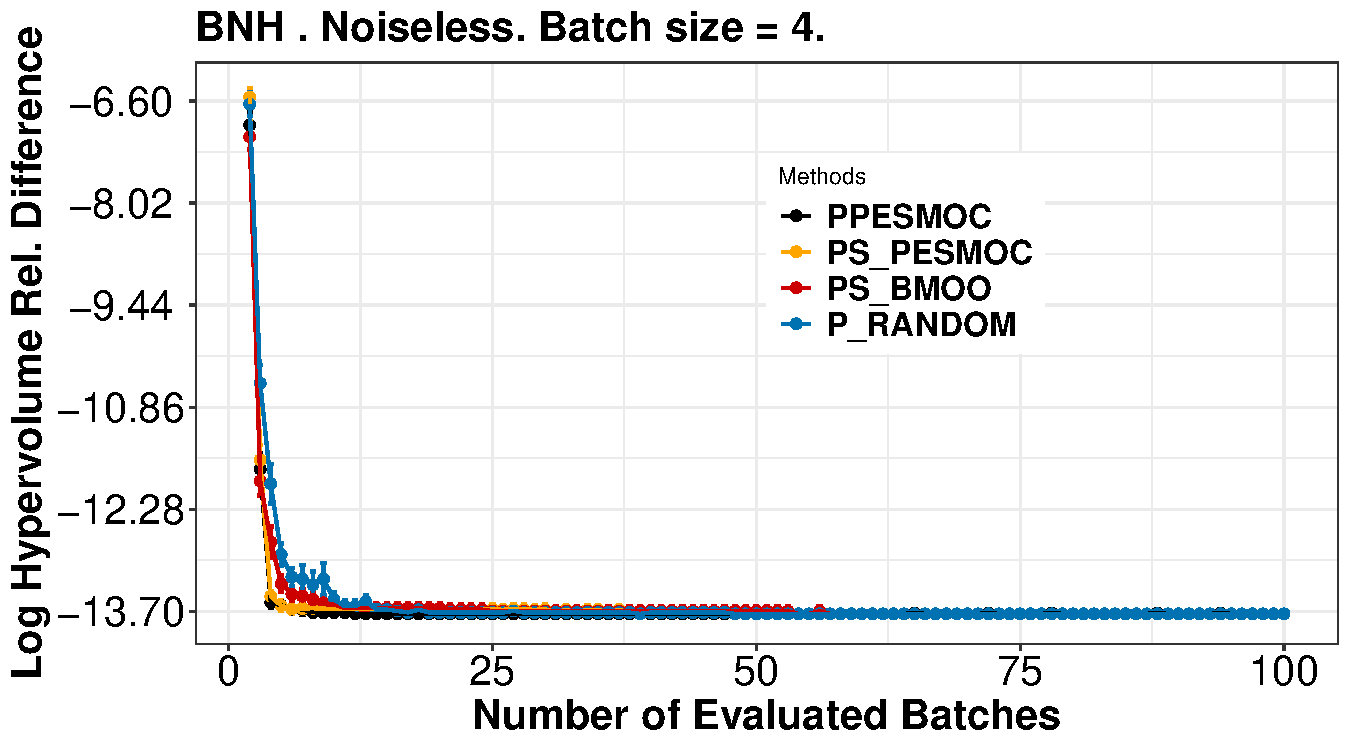
\includegraphics[width=0.49\textwidth]{Figures/ppesmoc/BNH.pdf}
\includegraphics[width=0.49\textwidth]{Figures/ppesmoc/SRN.pdf} \\
\includegraphics[width=0.49\textwidth]{Figures/ppesmoc/TNK.pdf}
\includegraphics[width=0.49\textwidth]{Figures/ppesmoc/TBT.pdf} \\
\includegraphics[width=0.49\textwidth]{Figures/ppesmoc/CONSTR.pdf}
\includegraphics[width=0.49\textwidth]{Figures/ppesmoc/OSY.pdf} \\
\caption{Logarithm of the relative difference between the hyper-volume of the recommendation obtained by each method and the hyper-volume of the actual solution. We report results after each evaluation of the black-box functions. Benchmark functions corrupted by noise.}
\label{fig:bench}
\end{center}
\end{figure}

\begin{figure}[ht]
        \begin{tabular}{cc}
                \includegraphics[width=0.475\linewidth]{Figures/ppesmoc/BNH_noisy.pdf} &
                \includegraphics[width=0.475\linewidth]{Figures/ppesmoc/SRN_noisy.pdf} \\
                \includegraphics[width=0.475\linewidth]{Figures/ppesmoc/TNK_noisy.pdf} &
                \includegraphics[width=0.475\linewidth]{Figures/ppesmoc/OSY_noisy.pdf} \\
                \includegraphics[width=0.475\linewidth]{Figures/ppesmoc/CONSTR_noisy_noisy.pdf} &
                \includegraphics[width=0.475\linewidth]{Figures/ppesmoc/TBT_noisy.pdf} 
        \end{tabular}
        \caption{{Average results for the problems BNH, SRN, TNK and OSY, CONSTR and TwoBar Truss. Noisy setting. }}
        \label{fig:benchmark_1}
\end{figure}

\subsection{Real-world Experiments}

We compare each method in the task of finding an optimal ensemble 
gradient-boosting ensemble. We consider two objectives: the prediction error of the
ensemble and its size. These objectives are conflictive since smaller ensembles 
will have in general higher error rates and the other way around. 
We introduce as a constraint of the problem, 
that the average speed up factor of the classification process given by a dynamic 
ensemble pruning technique  is at least 25$\%$ as we did in the previous chapter. We 
have carefully chosen this value to guarantee that the constraint is active at 
the optimal solution. The dataset considered is the German credit dataset extracted 
from the UCI repository \citep{Dua2019}. This is a binary classification dataset with $1,000$ 
instances and $20$ attributes. The prediction error is measured using 10-fold-cross validation, 
repeated 5 times. The ensemble size is the logarithm of the 
sum of the total number of nodes in the trees of the ensemble.

The adjustable parameters of the ensemble are: the number of trees 
(between 1 and $1,000$), the number of random attributes considered for split in 
each tree (between 1 and 20), the minimum number of samples required to split a node (between 2 and
200), the fraction of randomly selected training data used to build each tree (between 0.5 and 1.0),
and the fraction of training instances whose labels are changed after the sub-sampling process
(between $0.0$ and $0.7$).

Table \ref{table:ensemble_hypervolumes} shows the average hyper-volume obtained in this task, for each method, 
after $25$ and $50$ evaluations using a batch size of $4$. Figure \ref{fig:ensemble} (left) shows also the
average Pareto front obtained by each method. The Pareto front is simply given by the objective values 
associated to the recommendation made by each method. The higher the volume of points that is above this set
of points in the objective values the better the performance of a method. We observe that PPESMOC 
slightly outperforms the other approaches.
\begin{table}
\centering
\begin{tabular}{r@{$\pm$}l@{\hspace{.5cm}}r@{$\pm$}l@{\hspace{.5cm}}r@{$\pm$}l@{\hspace{.5cm}}r@{$\pm$}l}
\hline
\multicolumn{2}{c}{\bf PPESMOC} & \multicolumn{2}{c}{\bf PS\_PESMOC} & \multicolumn{2}{c}{\bf PS\_BMOO} & 
	\multicolumn{2}{c}{\bf P\_RANDOM} \\
\hline
\hspace{.5cm}\bf{0.231} & \bf{0.005} & \hspace{.5cm}0.228 & 0.005 & \hspace{.5cm} 0.228 & 0.008 & \hspace{.5cm}0.218 & 0.006 \\
\hline
\end{tabular}
\caption{Average hyper-volume in the task of finding an optimal ensemble of trees.}
\label{table:ensemble_hypervolumes}
\end{table}
As described in PESMOC,
we also evaluate each method on the task of finding an optimal deep neural network (DNN) on the 
MNIST dataset \citep{lecun2010mnist}. The objectives 
are the prediction error of the DNN on a validation 
dataset of $10,000$ instances (extracted from the original training set) and the time that such a DNN
will take for making predictions. These are conflictive objectives in the sense that 
minimizing the prediction error will often lead to bigger DNN with a bigger prediction times. 
We are also interested in codifying such a DNN into a chip.
Thus, we constrain the problem by enforcing that the area of the
resulting DNN, after being codified into a chip, is below $1$ $\text{mm}^2$.
We have carefully chosen this value to guarantee that the constraint is active at the optimal solution.
To measure the chip area we use the Aladdin simulator, which 
given a computer program describing the operations of the DNN, 
outputs an estimate of the area of a chip implementing those operations \citep{shao2014aladdin}.
To train the DNN we use the Keras library.
Prediction time is normalized by the smallest possible prediction time, which 
corresponds to a DNN of a single layer with $5$ hidden units.

\begin{figure}[ht]
\begin{center}
\begin{tabular}{cc}
\includegraphics[width=0.49\textwidth]{Figures/ppesmoc/plot_100_ensemble.pdf} & \includegraphics[width=0.49\textwidth]{Figures/ppesmoc/plot_200_ensemble.pdf} \\
\end{tabular}
\caption{Average Pareto front in the task of finding an optimal ensemble for 100 (left) and 200 evaluations (right).
}
\label{fig:ensemble}
\end{center}
\end{figure}

The input parameters to be optimized are:
The logarithm of the $\ell_1$  and $\ell_2$ weight regularizers;
the dropout probability; the logarithm of the initial learning
rate; the number of hidden units per layer; and the number of hidden layers. We have 
also considered two variables that have an impact in the hardware implementation
of the DNN. Namely, the logarithm (in base 2) of the array partition 
factor and the loop unrolling factor.
 
We report the performance after $15$ and $25$ evaluations using a batch 
size $B=4$. The DNN is trained  using ADAM with the default parameters. 
The loss function is the  cross-entropy. The last layer of 
the DNN contains 10 units and a soft-max activation function. All other layers use
Re-Lu as the activation function. Finally, each DNN is trained during a total of
$150$ epochs using mini-batches of size $4,000$.

\begin{figure}[ht]
\begin{center}
\begin{tabular}{cc}
\includegraphics[width=0.49\textwidth]{Figures/ppesmoc/plot_60_rrnn.pdf} & \includegraphics[width=0.49\textwidth]{Figures/ppesmoc/plot_100_rrnn.pdf} \\
\end{tabular}
\caption{Average Pareto front in the task of finding an optimal neural network for 60 (left) and 100 evaluations (right).
}
\label{fig:rrnn_op}
\end{center}
\end{figure}

The average Pareto front obtained by each method is shown in
Figure \ref{fig:rrnn_op}. Table \ref{table:aladdin_hypervolume} shows the 
average hyper-volume of each method. Here, PPESMOC outperforms by little 
PS\_PESMOC. PS\_BMOO gives worse results than PS\_PESMOC. The random search strategy
is the worst performing method. We can see in the frontier how the difference between the PPESMOC and PS\_PESMOC method is slight. PS\_PESMOC method suggests configurations with less prediction error and PPESMOC suggests neural networks with less energy consumption. 

\begin{table}
\centering
\caption{Hypervolume dominated by the proposed methods in the experiment. Larger hypervolume means better quality.}
\label{table:aladdin_hypervolume}
\begin{tabular}{r@{$\pm$}l@{\hspace{.5cm}}r@{$\pm$}l@{\hspace{.5cm}}r@{$\pm$}l@{\hspace{.5cm}}r@{$\pm$}l}
\hline
\multicolumn{2}{c}{\bf PPESMOC} & \multicolumn{2}{c}{\bf PS\_PESMOC} & \multicolumn{2}{c}{\bf PS\_BMOO} & 
	\multicolumn{2}{c}{\bf P\_RANDOM} \\
\hline
\hline
\hspace{.5cm}\bf{25.55} & \bf{0.03} & \hspace{.5cm}25.44 & 0.05 & \hspace{.5cm} 25.01 & 0.05 & \hspace{.5cm}24.61 & 0.03 \\
\hline
\end{tabular}
\end{table}

\section{Conclusions} \label{seq-conclusions}

In this chapter we have described PPESMOC, the first
method to address batch Bayesian optimization problems
with several objectives and constraints. More precisely,
PPESMOC suggests, at each iteration, at batch of
points at which the objectives and constraints should
be evaluated in parallel. We have compared the performance of PPESMOC
on several optimization problems, including synthetic, benchmark and real-world problems.
Furthermore, we have compared results with two simple base-lines.
Namely, a random exploration strategy and two methods derived
from the literature about sequential Bayesian optimization,
PS\_PESMOC and PS\_BMOO. We have observed that PPESMOC performs
well in general, giving similar and sometimes better results than PS\_PESMOC and PS\_BMOO.
The main advantage is, however, that the PPESMOC scales much better
with respect to the batch size. Unlike PPESMOC, the sequential strategies
require repeating an iterative process as many times as the batch size.
This process includes hallucinating observations, re-fitting the underlying GP models,
and optimizing a sequential acquisition function. This leads to
a prohibitive computational cost for large batch sizes.
